\section{Deep Neural Networks}
\label{section:cnn}
%PAPERS TO USE FOR CITING
%https://ieeexplore.ieee.org/abstract/document/6639344
%http://papers.nips.cc/paper/4824-imagenet-classification-with-deep-convolutional-neural-networ


%FIX decides whether to replace figures or not

A Neural Network (NN) is an interconnected group of nodes that follow a
computational model that propagates data forward while processing. The earliest
NNs were proposed by McCulloh and Pitts~\cite{neuron:model}, in which a neuron
has a linear part based on an aggregation of data, and then a non-linear part
called the activation function, which is applied to the aggregate sum. By aggregating several neurons in layers and the input of
each neuron as in Figure~\ref{MLP} being based on the previous layers, it can solve non-linear separable problems~\cite{approximation:problem}.

\begin{figure}[!htbp]
    \centering
    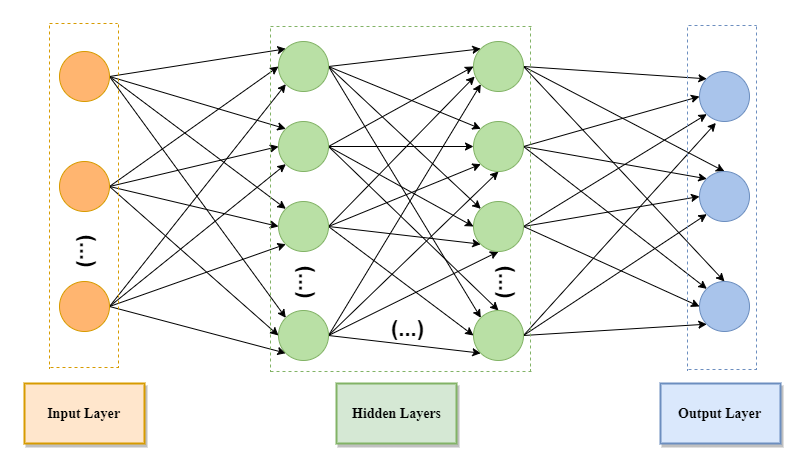
\includegraphics[width=0.8\textwidth]{Figures/mlp.png}
    \caption{Deep Neural Network Structure}
    \label{MLP}
\end{figure} 

Each input to a neuron contributes differently to the output. The share is
dependent on the weight value. These are obtained by training the network
through various techniques, one of which is called Deep Supervised
Learning~\cite{deeplearning} . For a certain input, there is an expected output
and the real output of the NN. Then the loss function (the difference) is
calculated, and the weight values are iteratively modified to improve the
outputs of the NN.

A Deep Neural Network (DNN) is a Neural Network that uses this approach for
learning. It has multiple hidden layers, and it can model complex non-linear
relationships. If the activation function is non-polynomial, it satisfies the
Universal approximation problem~\cite{approximation:problem}.

One of the limitations of traditional NNs is the complexity of layer
interconnections. Using as an example the hand digit recognition problem and MNIST
data set, composed of 28x28 grayscaled images~\cite{mnist:digits}, in a
traditional fully connected NN, a neuron from the second layer would have 28x28
weights. That is 3.136 kiloBytes per neuron of weight values while using 32-bit
floating-point numbers (FP32). When building a more complex network for image
recognition, the computational complexity grows quadratically with the number
of neurons per layer.

%One propriety of CNNs is the shift-invariance due to the use of 2D image convolution with filters and that makes them specifically
%good for Image and video recognition.

\subsection{Convolutional Neural Networks}
\label{section:subcnn}

Convolutional Neural Networks (CNN) are a class of DNNs used in Image and Video
recognition due to their shift invariance characteristic. They were first
proposed in the 1980s, but it was not until 2012 with AlexNet~\cite{alexnet} that
CNNs took off. Fundamentally, CNNs are a regularized version of
Multilayer Perceptrons (MLP). These networks fix the complexity issue discussed, as each neuron is only connected to a few neurons of the previous layer.
 

 \begin{figure}[!htbp]
    \centering
    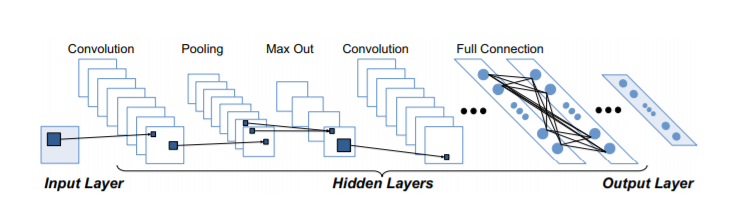
\includegraphics[width=1\textwidth]{Figures/convolutionlayer.png}
    \caption{CNN architecture example, taken from~\cite{cgracnn}}
    \label{CNNl}
\end{figure} 


 % There are several types of layers used in these networks to achieve the desired result.

 \paragraph{Convolutional Layer}
\label{section:convlayer}

In a typical CNN, not all layers are convolutional, but the convolutional layers
are the most compute-intensive. CNNs take input images with three  dimensions
(width, height, and color space); for the following convolutional layers, 3D
arrays are used (width, height, and number of channels). For the earlier example
of the MNIST data set, the input would have dimensions 28x28x1 as it is a 2D
image in grayscale.

To compute a neuron in the next layer, we use the convolution
Equation~\ref{equation:convolution} aided by Figure~\ref{Cl}.

\begin{equation} \label{equation:convolution}
   %\resizebox{.5 \textwidth}{!} 
    %%
\end{equation}
where $x_{j}^{l+1}$ is the output, $\delta$ is the activation function, which
depends on the architecture, $x_{i}^{l}$ is the input of the convolution layer,
$k_{ij}^{l+1}$ is the kernel of the said layer, which is obtained by training the
network, and $b_{j}^{l+1}$ is the bias.

Thus an output neuron depends only on a small region of the input, which is
called the local receptive field.

\begin{figure}[!htbp]
    \centering
    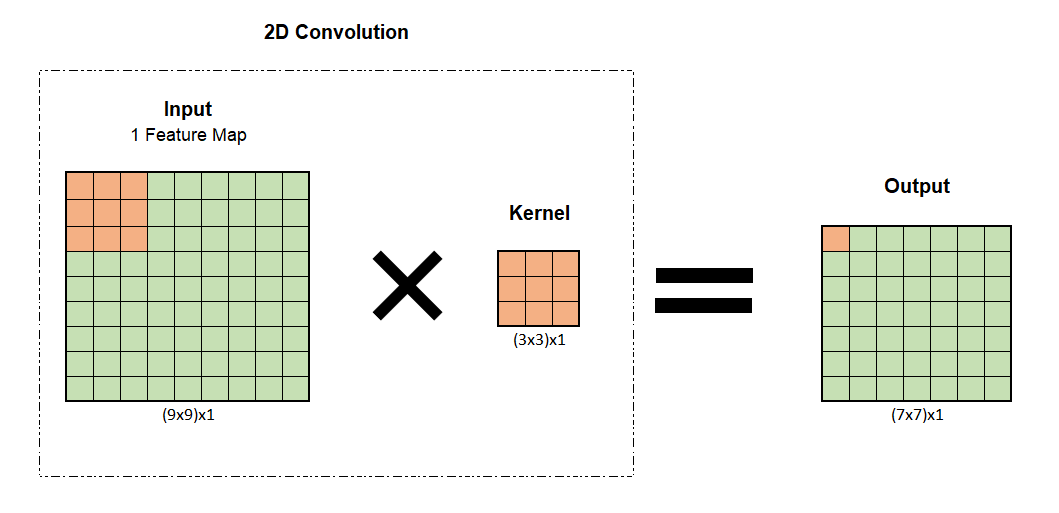
\includegraphics[width=1\textwidth]{Figures/conv.png}
    \caption{2D convolution with stride = one and without zero padding}
    \label{Cl}
\end{figure} 

The output's dimensions depend on convolution parameters such as
zero-padding and stride. The former means to add zeros around the edges of the
input matrix. The latter implies the step used for the convolution. If the value
is, e.g., 2, it will skip a pixel each iteration.
Equation~\ref{equation:padding} can be used to calculate the output spacial dimensionality\cite{cnnequation}.

\begin{equation} \label{equation:padding}
  \frac{(V-R)+2Z}{S+1}
\end{equation}
where $V$ is the input Volume, $R$ is the kernel size, $Z$ is the amount of zero-padding set while $S$ is the stride.

The number of channels of the output is equal to the number of filters in the
convolutional layer.

%Then a 3D convolution is performed with the kernel changing from layer to layer

\paragraph{Pooling Layer}

The MaxPool or AvgPool are layers used in Convolutional Neural Networks to
downsampling the feature maps to make the output maps less sensitive to the
location of the features.

Maximum Pooling or MaxPool, like is suggested in its name groups $ n * n $
points and outputs the pixel with the highest value.  The output will have its size
lowered by $n$ times.  The Average Pooling or AvgPool, instead takes all of
the input points and calculates the average. Downsampling can also be achieved
by using convolutions with stride two and padding equal to 1.  Upsample layers can
also be utilized that turn each pixel into $n^{2}$, where $n$ is the number of times
the output will be bigger than the input.

\begin{figure}[!htbp]
    \centering
    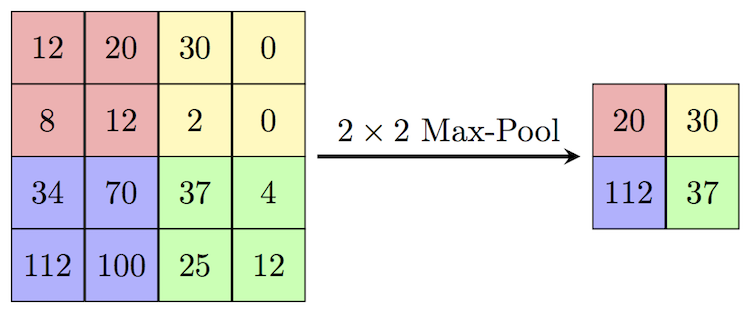
\includegraphics[width=0.5\textwidth]{Figures/maxpool.png}
    \caption{Simple example of a max pool layer, taken from~\cite{maxpoolimg}}
    \label{figure:maxpool}
\end{figure} 
 

\paragraph{Fully Connected Layer}

The fully connected layer is mainly used for classification in the final layers
of the NN. It associates the feature map with the respective labels.  It takes the
3D vector and outputs a single vector. Thus, it is also known as flatten.
Equation~\ref{equation:connected} describes the operation.

\begin{equation} \label{equation:connected}
    %\resizebox{.5 \textwidth}{!} 
     %%
\end{equation}
where $w_{ji}^{l+1}$ are the weights associated with a specific input for each output.


\paragraph{Route $\&$ Shortcut Layer}

The Shortcut layer or skip connection was first introduced in
Resnet~\cite{resnet}.  It allows connecting of the previous layer to another to
allow the flow of information across layers.  The Route layer, used in
Yolov3~\cite{yolov3}, concatenates two layers in depth (channel) or skips the
layer forward. This is used after the detection layer in Yolov3 to extract other
features.

\paragraph{Dropout Layer}

This type of layer was conceived to avoid overfitting~\cite{Dropout} by dropping
the neurons with a probability below the threshold. In Figure~\ref{figure:Dropout}, there is a graphical representation.
\begin{figure}[!htbp]
    \centering
    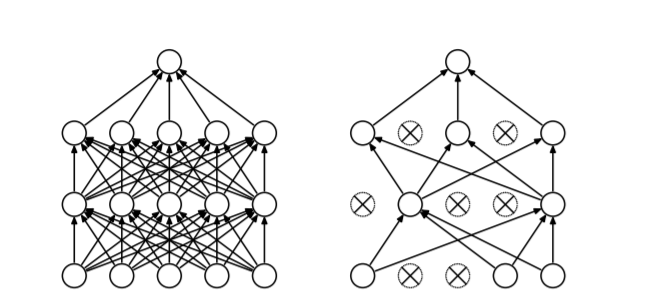
\includegraphics[width=0.6\textwidth]{Figures/dropout.png}
    \caption{Dropout if applied to all layers, adapted from~\cite{Dropout}}
    \label{figure:Dropout}
\end{figure} 

\paragraph{Activation Functions}

Activation Functions (AF) are functions used in each layer of a NN
to compute the weighted sum of input and biases, which is used to give a value
to a neuron. Non-linear AFs are used to transform linear inputs into non-linear
outputs.  While training Deep Neural Networks, vanishing and exploding
gradients are common issues. In other words, after successive multiplications
of the loss gradient, the values tend to zero or infinity, and thus, the
gradient disappears. AFs help mitigate this issue by keeping the gradient within
specific limits. The most popular activation functions can be found in
Table~\ref{table:AF}.

\begin{table}[]
    \centering
    \resizebox{.6\textwidth}{!}{%}
    \begin{tabular}{ll}
    \hline
    \textbf{Activation Functions} & \textbf{Computation Equation} \\ \hline \hline
    Sigmoid                       &  $\displaystyle f(x)=\frac{1}{1+ e^{-x}}$                             \\ \hline
    Tanh                          &  $\displaystyle f(x)=\frac{e^{x}-e^{-x}}{e^{x}+e^{-x}}$                            \\ \hline
    Softmax                       &  $\displaystyle f(x_{i})=\frac{x_{i}}{\sum_{j}e^{x_{j}}}$                             \\ \hline
    ReLU                          &    $ f(x)=\begin{matrix}
        x & if & x\geq 0  \\ 
        0 & if & x< 0 
    \end{matrix} $                           \\ \hline
    LReLU                         &  $f(x)= \begin{matrix}
        x & if & x > 0  \\ 
        \alpha x & if & x \leq 0 
    \end{matrix} $                        \\ \hline
    ELU                           &             $ f(x)=\begin{matrix}
        x & if & x> 0  \\ 
        \alpha e^{x} - 1 & if & x\leq 0 
    \end{matrix} $                 \\ \hline
    \end{tabular}%
    }
    \caption{Popular activation functions}
    \label{table:AF}
\end{table}


%image of activation functions?

 \subsection{Frameworks for Neural Networks}
 \label{section:Darknet}

To run a Neural Network model, there are several popular frameworks like
Tensorflow, PyTorch, Caffe, and Darknet.  They aim to offer abstraction
to software developers who want to run these networks. They also provide
programming for platforms like Nvidia GPUs using the CUDA API.

\subsubsection{Darknet}

Darknet~\cite{Darknet} is an open-source neural network framework written in C
and CUDA. It is the backbone for Yolov3~\cite{yolov3} and supports
several network configurations, such as AlexNet and Resnet.  It
utilizes a network configuration file (.cfg) and a weights file (.weights) as
input for inference.

\lstinputlisting[label=cfg,language=Python,frame=single,breaklines=true,firstline=13,lastline=19,caption=cfg
  code for a Convolutional Layer used in
  Yolov3~\cite{yolov3}]{./Code/yolov3.cfg}

In Listing~\ref{cfg}, there is a snippet of the file featuring a convolution
layer with 32 kernels of size 3x3. It has stride one and zero padding of 1,
meaning the output size equals the input size. The input size can be
calculated by analyzing the previous layers and the network parameters. The
network parameters in Listing~\ref{net} include data for training, while only
the first three parameters are needed for inference.

\lstinputlisting[label=net,language=Python,frame=single,breaklines=true,firstline=1,lastline=11,caption=cfg
  code for the network parameters]{./Code/yolov3.cfg}


\subsubsection{Caffe}

Convolutional Architecture for Fast Feature Embedding (Caffe)~\cite{caffe} is
also an open-source framework written in C++ with a Python interface.  Caffe
exports a neural network by serializing it using the Google Protocol Buffers
(ProtoBuf) serialization library. Each network has two prototxt files:
\begin{itemize}
    \item deploy.prototxt- File that describes the network structure that
      can be deployed for inference.
    \item train\_val.prototxt- File that includes structure for training.  It
      includes the extra layers used to aid the training and validation process.
\end{itemize}

The Python interface helps generate these files. For inference, only the
deploy file matters. In Listing~\ref{caffe}, there is a snippet of a deployed file. 

\lstinputlisting[label=caffe,language=Python,frame=single,breaklines=true,firstline=1,lastline=26,caption=prototxt
  file for the input data and the first convolution layer of
  AlexNet~\cite{alexnet}]{./Code/caffe.prototxt}
